\documentclass[letterpaper,11pt]{article}

%packages
\usepackage{amsfonts}
\usepackage{graphicx}
\usepackage[left=2cm,top=2cm,right=2cm,bottom=2cm,head=.5cm,foot=.5cm]{geometry}
\usepackage{url}
\usepackage{multirow}
\usepackage{longtable}
\usepackage{subfig}
\usepackage{float}
\usepackage{setspace}
\usepackage{lineno}
\usepackage{natbib}
\usepackage{amsmath}
\usepackage{xr}
\usepackage{authblk}

%new commands and so on
\providecommand{\keywords}[1]
{
  \small	
  \textbf{\textit{Keywords---}} #1
}

%external documents
\externaldocument[SM-]{SupMat}
 
%header material for paper
\title{Place title here}
\date{}

\author[a]{Jasmin Albert}
\author[a,b]{Daniel C. Reuman}

\affil[a]{Department of Ecology and Evolutionary Biology and Kansas Biological Survey, University of Kansas}
\affil[b]{Laboratory of Populations, Rockefeller University}

%***Need to indicate corresponding authors

\usepackage{Sweave}
\begin{document}
\Sconcordance{concordance:Paper.tex:Paper.Rnw:%
1 55 1 50 0 1 7 75 1}


%The following is where you load in the numeric results that will be embedded in the text

\maketitle

\begin{abstract}
Place abstract here
\end{abstract}

%***Add to these
\keywords{kw1, kw2,kw3}

\section{Introduction}\label{section:introduction}


\section{Methods}\label{section:methods}


\section{Results}\label{section:results}


\section{Discussion}\label{section:discussion}


\section{Reference code for Jasmin to learn Latex/Sweave}

To get normal text you just type.

To get a paragraph break you leave a blank line, indentation is automatic.

\noindent If you want to remove the indent you use this.

In-line math is always surrounded by dollar signs, $x+1=4$. Even when you just have single variables, like if you say ``the notation we use for synchrony is $x$'', you put the $x$ in dollar signs. The reason is x and $x$ look different, in a way that a mathematician will notice and wonder if they are meant to be different variables.

For quotes, do it ``like this'' not "like this" or else one of the quotes will be backwards.

Some basic math, inline, by example: $x_{11}$, $y^{22}$, $\frac{1+y}{x+3}$, $\sum_{i=1}^N x_x$,
$\alpha$, $\beta$.

There is also display math:
\begin{equation}
x=y+12-z \label{eq_about_x_and_y}
\end{equation}
The ``label'' command allows a textual label for refering to equations later.

The math gets pretty complex. Keep in mind, whatever you want to do, there is a way to do it. We'll save most of that for later.

Now we can refer to equation/expression (\ref{eq_about_x_and_y}). Latex will sort
out equation numbering and insert the correct number labels for you.

You can also refer to any section in the same way: section \ref{section:introduction}, section \ref{section:methods}.

You can include the value of previously loaded R variables in the text, e.g., the value of allregres[1,5] is
-1.16948109243002, which can also be given rounded: -1.169. You can do simple R
on the fly, e.g., allregres[1,5] plus 1 is -0.169481092430019. 
You should never manually type any results, they should always be autolinks like this.

%Comments are lines starting with %

You make a percent with \%

You can refer to Fig. \ref{fig:random_fig} by its label and latex will number figures and use the correct numbers.
The label is defined below where the figure is placed.

You can refer to Table \ref{tab:random_table} in the same way.

%You can also refer to figures and tables and equations from the sup mat, just prefix the labels
%by SM- in your calls to \ref{}

You can cite like this \cite{Abanetal2006} or this \citep{Abanetal2006} or this \citealp{Abanetal2006}.
You cal also cite books \citep{BurnhamAnderson2002}, of course.

\clearpage
\newpage

%you store your bibliographic info in refs.bib, see that file
\bibliographystyle{ecology_letters2}
\bibliography{refs}

\clearpage
\newpage

\section{Tables}

%You make tables like this:
\begin{table}[H]
\caption[Summary caption, for table of contents, can be skipped.]{Full caption here.}
\begin{tabular}{llll} %The four ls mean four columns, each left justified. Can use r or c, too.
\hline 
Col 1 header & Col 2 header & Col 3 header & Col 4 header \\
\hline
text & or & numbers & 3.2 \\
or & math & $x+1$ & or \\
even & the & values & of \\
loaded & R & variables & -1.16948109243002 \\
you & can & round & -1.169 \\ 
\hline
\end{tabular}
\label{tab:random_table}
\end{table}

\clearpage
\newpage


\section{Figures}

\begin{figure}[!h]
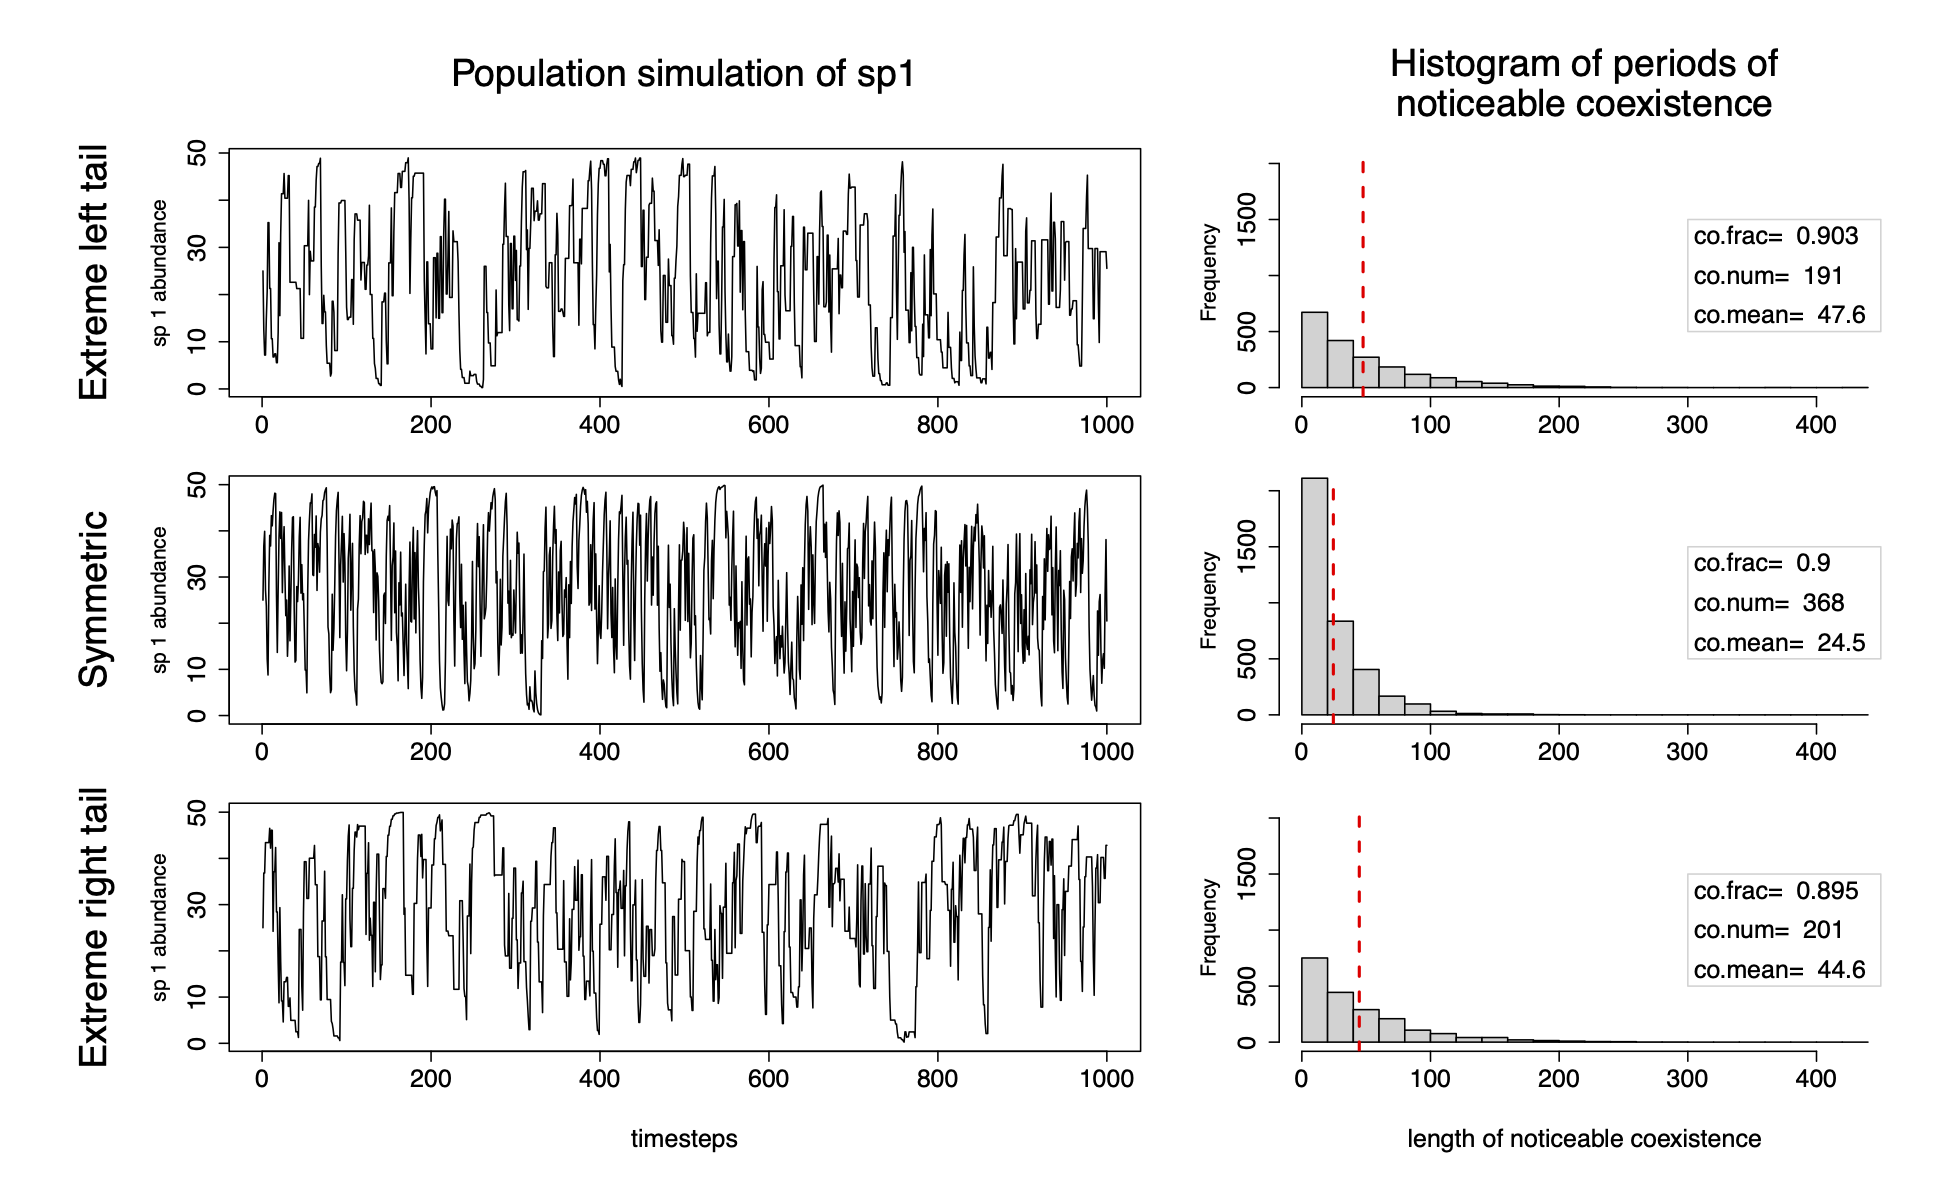
\includegraphics[width=.5\textwidth]{figures/summaryDocFigures/figure8.png}
\caption{Type the caption here.} \label{fig:random_fig}
\end{figure}


\end{document}
